% ncse_new/p1_SystemsOfEquations/ch2_DirectMethodsLSE/ex_circuitimpedance.tex
% require: rcircuit.eps 
% Picture directory: /u/hiptmair/NOSAVE/numpde/Numcourses/ncse/ncse_new/EXERCISES/AS15/Problems/ch_directmethodslse/PICTURES
\renewcommand{\chpt}{ch_directmethodslse}

\begin{problem}[Resistance to impedance map]\label{prb:cimp}
  In \lref{par:smw}, we learned about the Sherman-Morrison-Woodbury update formula
  \lref{lem:SMW}, which allows the efficient solution of a linear system of
  equations after a low-rank update according to \lref{mod:1}, provided that the
  setup phase of an elimination ($\to$ \lref{alg:LULSE}) solver has already been
  done for the system matrix.

  In this problem, we examine the concrete application from \lref{ex:rcircuit}, where
  the update formula is key to efficient implementation. This application is the 
  computation of the impedance of the circuit drawn in Figure~\ref{fig:rcircuit} 
  as a function of a variable resistance of a \emph{single} circuit element.

  \begin{figure}[h]
    \centering
    % \psfrag{L1}[l][l]{\small {$L$}}
    % \psfrag{R1}{\small {$R$}}
    % \psfrag{R2}[c][c]{\small {$R$}}
    % \psfrag{C1}{\small {$C_{1}$}}
    % \psfrag{C2}{\small {$C_{2}$}}
    % \psfrag{R3}{\small {$R$}}
    % \psfrag{R4}{\small {$R$}}
    % \psfrag{R5}[c][c]{\small {$R$}}
    % \psfrag{Rx}{{$R_{x}$}}
   %  \psfrag{1}{}
   %  \psfrag{2}{}
   %  \psfrag{3}{}
   %  \psfrag{4}{}
   %  \psfrag{5}{}
   %  \psfrag{6}{}
   % \psfrag{7}{}
   %  \psfrag{8}{}
   %  \psfrag{9}{}
   %  \psfrag{10}{}
   %  \psfrag{11}{}
   %  \psfrag{13}{}
   %  \psfrag{14}{}
   %  \psfrag{15}{}
   %  \psfrag{16}{}
   %  \psfrag{17}{}
   %  \psfrag{18}{}
    \psfrag{U}{{$U$}}
    \psfrag{Rx}{\Magenta{$R_{x}$}}
    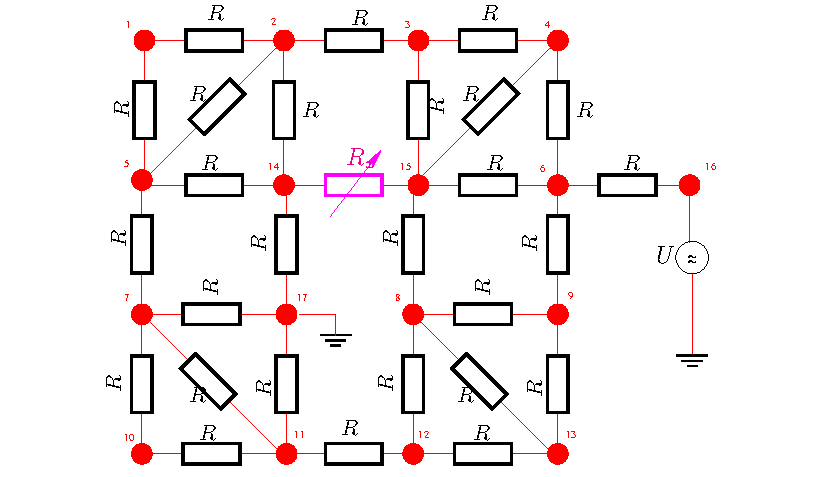
\includegraphics[width=0.9\textwidth]{\problems/\chpt/PICTURES/rcircuit_convert.pdf}
    \caption{Resistor circuit with a single controlled resistance}
    \label{fig:rcircuit}
  \end{figure}
  

\begin{subproblem}[2]\label{cimp:sp:1}
  Study \lref{ex:elnet} that explains how to compute voltages and currents in a
  linear circuit by means of nodal analysis. Understand how this leads to a linear
  system of equations for the unknown nodal potentials. The fundamental laws of
  circuit analysis should be known from physics as well as the principles of nodal
  analysis.
\end{subproblem}

\begin{subproblem}[3]\label{cimp:sp:2}
  Use nodal analysis to derive the linear system of equations satisfied by 
  the nodal potentials of the circuit from Figure~\ref{fig:rcircuit}. 
  The voltage $W$ is applied to node \#16 and node \#17 is grounded. 
  All resistors except for the controlled one (colored magenta) 
  have the same resistance $R$.
  Use the numbering of nodes indicated in Figure~\ref{fig:rcircuit}.
  
  \begin{hint}
    Optionally, you can make the computer work for you and find a fast way to build
    a matrix providing only the essential data. This is less tedious, less error
    prone and more flexible than specifying each entry individually. For this you
    can use auxiliary data structures.
  \end{hint}
  
  \begin{solution}
   We use the Kirchhoff's first law (as in \lref{ex:elnet}), stating that the sum the currents incident to a node is zero. Let $\vec{W} \in \IR^{17}$ be the vector of voltages. Set $f(R_x) := R / R_x$. We rescale each sum multiplying by $R$. Let us denote by $\Delta W_{i,j} := (W_i - W_j)$. The system  for each node $i = 1,\dots,15$ becomes: 
   \begin{align} \label{eq:syst_impedance}
   \begin{cases} 
    \Delta W_{1,2} + \Delta W_{1,5} & = 0 \\
    \Delta W_{2,1} + \Delta W_{2,3} + \Delta W_{2,5} + \Delta W_{2,14} & = 0 \\
    \Delta W_{3,2} + \Delta W_{3,4} + \Delta W_{3,15} & = 0 \\
    \Delta W_{4,3} + \Delta W_{4,6} + \Delta W_{4,15} & = 0 \\
    \Delta W_{5,1} + \Delta W_{5,2} + \Delta W_{5,7} + \Delta W_{5,14} & = 0 \\
    \Delta W_{6,4} + \Delta W_{6,9} + \Delta W_{6,15} + \Delta W_{6,16} & = 0 \\
    \Delta W_{7,5} + \Delta W_{7,10} + \Delta W_{7,11} + \Delta W_{7,17} & = 0 \\
    \Delta W_{8,9} + \Delta W_{8,12} + \Delta W_{8,13} + \Delta W_{8,5} & = 0 \\
    \Delta W_{9,6} + \Delta W_{9,8} + \Delta W_{9,13} & = 0 \\
    \Delta W_{10,7} + \Delta W_{10,11} & = 0 \\
    \Delta W_{11,7} + \Delta W_{11,10} + \Delta W_{11,12} + \Delta W_{11,17} & = 0 \\
    \Delta W_{12,8} + \Delta W_{12,11} + \Delta W_{12,13} & = 0 \\
    \Delta W_{13,8} + \Delta W_{13,9} + \Delta W_{13,12} & = 0 \\
    \Delta W_{14,2} + \Delta W_{14,5} + \Delta W_{14,17} + f(R_x) \Delta W_{14,15} & = 0 \\
    \Delta W_{15,3} + \Delta W_{15,4} + \Delta W_{15,6} + \Delta W_{15,8} + f(R_x) \Delta W_{15,14} & = 0
   \end{cases}
   \end{align}
   with the extra condition $W_{16} := W, W_{17} = 0$. We now have to obtain the system matrix. The system is rewritten in the following matrix notation (with $\vec{C} \in \IR^{15,17}$):
   \[
    \vec{C} = [\vec{A}(R_x), \vec{B}] \vec{W} = \vec{0} \; \Leftrightarrow \; \vec{A}(R_x) \tilde{\vec{W}} = - \vec{B} \cdot [W_{16}, \; W_{17}]^\top =: rhs
   \]
   with $\vec{W} = [\vec{\tilde{W}}, \; W_{16}, \; W_{17}]$, and with:
   \setcounter{MaxMatrixCols}{20}
   \begin{align*}
    \vec{A}(R_x) = \begin{bmatrix} 
      2 & -1 & 0 & 0 & -1 & 0 & 0 & 0 & 0 & 0 & 0 & 0 & 0 & 0 & 0 \\
      -1 & 4 & -1 & 0 & -1 & 0 & 0 & 0 & 0 & 0 & 0 & 0 & 0 & -1 & 0 \\
      0 & -1 & 3 & -1 & 0 & 0 & 0 & 0 & 0 & 0 & 0 & 0 & 0 & 0 & -1 \\
      0 & 0 & -1 & 3 & 0 & -1 & 0 & 0 & 0 & 0 & 0 & 0 & 0 & 0 & -1 \\
      -1 & -1 & 0 & 0 & 4 & 0 & -1 & 0 & 0 & 0 & 0 & 0 & 0 & -1 & 0 \\
      0 & 0 & 0 & -1 & 0 & 4 & 0 & 0 & -1 & 0 & 0 & 0 & 0 & 0 & -1 \\
      0 & 0 & 0 & 0 & -1 & 0 & 4 & 0 & 0 & -1 & -1 & 0 & 0 & 0 & 0 \\
      0 & 0 & 0 & 0 & 0 & 0 & 0 & 4 & -1 & 0 & 0 & -1 & -1 & 0 & -1 \\
      0 & 0 & 0 & 0 & 0 & -1 & 0 & -1 & 3 & 0 & 0 & 0 & -1 & 0 & 0 \\
      0 & 0 & 0 & 0 & 0 & 0 & -1 & 0 & 0 & 2 & -1 & 0 & 0 & 0 & 0 \\
      0 & 0 & 0 & 0 & 0 & 0 & -1 & 0 & 0 & -1 & 4 & -1 & 0 & 0 & 0 \\
      0 & 0 & 0 & 0 & 0 & 0 & 0 & -1 & 0 & 0 & -1 & 3 & -1 & 0 & 0 \\
      0 & 0 & 0 & 0 & 0 & 0 & 0 & -1 & -1 & 0 & 0 & -1 & 3 & 0 & 0 \\
      0 & -1 & 0 & 0 & -1 & 0 & 0 & 0 & 0 & 0 & 0 & 0 & 0 & 3 + \frac{R}{R_x} & -\frac{R}{R_x} \\
      0 & 0 & -1 & -1 & 0 & -1 & 0 & -1 & 0 & 0 & 0 & 0 & 0 & -\frac{R}{R_x} & 4 + \frac{R}{R_x} \\
        \end{bmatrix} \\
   \end{align*}
    a square $15 \times 15$ matrix and $\vec{B} \in \IR^{15,2}$ zero except $B_{6,1} = -R$.

   (For each term with the form $\beta \cdot \Delta W_{i,j}$ in \eqref{eq:syst_impedance} we have add an entry $\beta$ in the diagonal $i,i$ and an entry $-\beta$ in the cell $i,j$ (if $j \leq 15$). Entries with $j > 15$ will produce a corresponding positive entry $\beta \cdot U_j$ in the r.h.s.)
  \end{solution}

\end{subproblem}

\begin{subproblem}[3]\label{cimp:sp:3}
  Characterize the change in the circuit matrix derived in
  sub-problem~\ref{cimp:sp:2} induced by a change in the value of $R_{x}$ 
  as a low-rank modification of the circuit matrix. Use as a base state $R = R_x$.

  \begin{hint}
    Four entries of the circuit matrix will change. This amounts to
    a rank-2-modification in the sense of \lref{mod:1} with suitable
    matrices $\Vu$ and $\Vv$. 
  \end{hint}
  
  \begin{solution}
   The matrices
   \begin{align*}
    \vec{U} = \begin{bmatrix}
               0 & 0 \\
               \vdots & \vdots \\
               -1 & 1 \\
               1 & -1
              \end{bmatrix} = \vec{V}
   \end{align*}
   are such that $\vec{A}(R)$ defined as $\vec{A}(R_x)$ allows to write:
   \begin{align*}
    \vec{A}(R_x) = \vec{A}(R) - \vec{U} \vec{V^\top} \left(1 - \frac{R}{R_x} \right) / {2}.
   \end{align*}
   Therefore, if we already have the factorization of $\vec{A}_0$, we can use the SMW formula for the cheap inversion of $\vec{A}(R_x)$.
\end{solution}

\end{subproblem}

\begin{subproblem}[3]
  Based on the \eigen{} library, implement a C++ class 
\begin{lstlisting}[style=cppsimple]
class ImpedanceMap {
public:
  ImpedanceMap(double R_, double W_) : R(R_), W(W_) {
      // TODO: build A0 = A(1), the rhs and factorize A\_0 with lu = A0.lu()
  };
  double operator() (double Rx) const {
      // TODO: compute the perturbation matrix U and solve ($A + UU^T$) x = rhs, from x, U and R compute the impedance
  };
private:
  Eigen::PartialPivLU<Eigen::MatrixXd>> lu;
  Eigen::VectorXd rhs;
  double R, W;
};   
\end{lstlisting}
whose \texttt{()}-operator returns the impedance of the circuit from 
Figure~\ref{fig:rcircuit} when supplied with a concrete value for $R_{x}$.
Of course, this function should be implemented efficiently using 
\lref{lem:SMW}. The setup phase of Gaussian elimination should be carried
out in the constructor performing the LU-factorization of the circuit matrix.

Test your class using $R = 1, W = 1$ and $R_x=1,2,4,\cdots,1024$.
\begin{hint}
 See the file \texttt{impedancemap.cpp}.
\end{hint}

\begin{hint}
  The impedance of the circuit is the quotient of the voltage at the
  input node \#16 and the current through the voltage source.
\end{hint}

% \begin{hint}
%  Remember Ohm's law $I = \Delta V / R$.
% \end{hint}

\end{subproblem}


\end{problem}
